\documentclass[a4paper,12pt,twoside]{memoir}

% Castellano
\usepackage[spanish,es-tabla]{babel}
\selectlanguage{spanish}
\usepackage[utf8]{inputenc}
\usepackage[T1]{fontenc}
\usepackage{lmodern} % scalable font
\usepackage{microtype}
\usepackage{placeins}

\RequirePackage{booktabs}
\RequirePackage[table]{xcolor}
\RequirePackage{xtab}
\RequirePackage{multirow}

% Links
\usepackage[colorlinks]{hyperref}
\hypersetup{
	allcolors = {red}
}

% Ecuaciones
\usepackage{amsmath}

% Rutas de fichero / paquete
\newcommand{\ruta}[1]{{\sffamily #1}}

% Párrafos
\nonzeroparskip


% Imagenes
\usepackage{graphicx}
\newcommand{\imagen}[2]{
	\begin{figure}[!h]
		\centering
		\includegraphics[width=0.9\textwidth]{#1}
		\caption{#2}\label{fig:#1}
	\end{figure}
	\FloatBarrier
}

\newcommand{\imagenflotante}[2]{
	\begin{figure}%[!h]
		\centering
		\includegraphics[width=0.9\textwidth]{#1}
		\caption{#2}\label{fig:#1}
	\end{figure}
}



% El comando \figura nos permite insertar figuras comodamente, y utilizando
% siempre el mismo formato. Los parametros son:
% 1 -> Porcentaje del ancho de página que ocupará la figura (de 0 a 1)
% 2 --> Fichero de la imagen
% 3 --> Texto a pie de imagen
% 4 --> Etiqueta (label) para referencias
% 5 --> Opciones que queramos pasarle al \includegraphics
% 6 --> Opciones de posicionamiento a pasarle a \begin{figure}
\newcommand{\figuraConPosicion}[6]{%
  \setlength{\anchoFloat}{#1\textwidth}%
  \addtolength{\anchoFloat}{-4\fboxsep}%
  \setlength{\anchoFigura}{\anchoFloat}%
  \begin{figure}[#6]
    \begin{center}%
      \Ovalbox{%
        \begin{minipage}{\anchoFloat}%
          \begin{center}%
            \includegraphics[width=\anchoFigura,#5]{#2}%
            \caption{#3}%
            \label{#4}%
          \end{center}%
        \end{minipage}
      }%
    \end{center}%
  \end{figure}%
}

%
% Comando para incluir imágenes en formato apaisado (sin marco).
\newcommand{\figuraApaisadaSinMarco}[5]{%
  \begin{figure}%
    \begin{center}%
    \includegraphics[angle=90,height=#1\textheight,#5]{#2}%
    \caption{#3}%
    \label{#4}%
    \end{center}%
  \end{figure}%
}
% Para las tablas
\newcommand{\otoprule}{\midrule [\heavyrulewidth]}
%
% Nuevo comando para tablas pequeñas (menos de una página).
\newcommand{\tablaSmall}[5]{%
 \begin{table}
  \begin{center}
   \rowcolors {2}{gray!35}{}
   \begin{tabular}{#2}
    \toprule
    #4
    \otoprule
    #5
    \bottomrule
   \end{tabular}
   \caption{#1}
   \label{tabla:#3}
  \end{center}
 \end{table}
}

%
%Para el float H de tablaSmallSinColores
\usepackage{float}

%
% Nuevo comando para tablas pequeñas (menos de una página).
\newcommand{\tablaSmallSinColores}[5]{%
 \begin{table}[H]
  \begin{center}
   \begin{tabular}{#2}
    \toprule
    #4
    \otoprule
    #5
    \bottomrule
   \end{tabular}
   \caption{#1}
   \label{tabla:#3}
  \end{center}
 \end{table}
}

\newcommand{\tablaApaisadaSmall}[5]{%
\begin{landscape}
  \begin{table}
   \begin{center}
    \rowcolors {2}{gray!35}{}
    \begin{tabular}{#2}
     \toprule
     #4
     \otoprule
     #5
     \bottomrule
    \end{tabular}
    \caption{#1}
    \label{tabla:#3}
   \end{center}
  \end{table}
\end{landscape}
}

%
% Nuevo comando para tablas grandes con cabecera y filas alternas coloreadas en gris.
\newcommand{\tabla}[6]{%
  \begin{center}
    \tablefirsthead{
      \toprule
      #5
      \otoprule
    }
    \tablehead{
      \multicolumn{#3}{l}{\small\sl continúa desde la página anterior}\\
      \toprule
      #5
      \otoprule
    }
    \tabletail{
      \hline
      \multicolumn{#3}{r}{\small\sl continúa en la página siguiente}\\
    }
    \tablelasttail{
      \hline
    }
    \bottomcaption{#1}
    \rowcolors {2}{gray!35}{}
    \begin{xtabular}{#2}
      #6
      \bottomrule
    \end{xtabular}
    \label{tabla:#4}
  \end{center}
}

%
% Nuevo comando para tablas grandes con cabecera.
\newcommand{\tablaSinColores}[6]{%
  \begin{center}
    \tablefirsthead{
      \toprule
      #5
      \otoprule
    }
    \tablehead{
      \multicolumn{#3}{l}{\small\sl continúa desde la página anterior}\\
      \toprule
      #5
      \otoprule
    }
    \tabletail{
      \hline
      \multicolumn{#3}{r}{\small\sl continúa en la página siguiente}\\
    }
    \tablelasttail{
      \hline
    }
    \bottomcaption{#1}
    \begin{xtabular}{#2}
      #6
      \bottomrule
    \end{xtabular}
    \label{tabla:#4}
  \end{center}
}

%
% Nuevo comando para tablas grandes sin cabecera.
\newcommand{\tablaSinCabecera}[5]{%
  \begin{center}
    \tablefirsthead{
      \toprule
    }
    \tablehead{
      \multicolumn{#3}{l}{\small\sl continúa desde la página anterior}\\
      \hline
    }
    \tabletail{
      \hline
      \multicolumn{#3}{r}{\small\sl continúa en la página siguiente}\\
    }
    \tablelasttail{
      \hline
    }
    \bottomcaption{#1}
  \begin{xtabular}{#2}
    #5
   \bottomrule
  \end{xtabular}
  \label{tabla:#4}
  \end{center}
}



\definecolor{cgoLight}{HTML}{EEEEEE}
\definecolor{cgoExtralight}{HTML}{FFFFFF}

%
% Nuevo comando para tablas grandes sin cabecera.
\newcommand{\tablaSinCabeceraConBandas}[5]{%
  \begin{center}
    \tablefirsthead{
      \toprule
    }
    \tablehead{
      \multicolumn{#3}{l}{\small\sl continúa desde la página anterior}\\
      \hline
    }
    \tabletail{
      \hline
      \multicolumn{#3}{r}{\small\sl continúa en la página siguiente}\\
    }
    \tablelasttail{
      \hline
    }
    \bottomcaption{#1}
    \rowcolors[]{1}{cgoExtralight}{cgoLight}

  \begin{xtabular}{#2}
    #5
   \bottomrule
  \end{xtabular}
  \label{tabla:#4}
  \end{center}
}




\graphicspath{ {./img/} }

% Capítulos
\chapterstyle{bianchi}
\newcommand{\capitulo}[2]{
	\setcounter{chapter}{#1}
	\setcounter{section}{0}
	\chapter*{#2}
	\addcontentsline{toc}{chapter}{#2}
	\markboth{#2}{#2}
}

% Apéndices
\renewcommand{\appendixname}{Apéndice}
\renewcommand*\cftappendixname{\appendixname}

\newcommand{\apendice}[1]{
	%\renewcommand{\thechapter}{A}
	\chapter{#1}
}

\renewcommand*\cftappendixname{\appendixname\ }

% Formato de portada
\makeatletter
\usepackage{xcolor}
\newcommand{\tutor}[1]{\def\@tutor{#1}}
\newcommand{\course}[1]{\def\@course{#1}}
\definecolor{cpardoBox}{HTML}{E6E6FF}
\def\maketitle{
  \null
  \thispagestyle{empty}
  % Cabecera ----------------
\noindent
\includegraphics[width=\textwidth]{cabecera}\vspace{1cm}%
  \vfill
  % Título proyecto y escudo informática ----------------
  \colorbox{cpardoBox}{%
    \begin{minipage}{.8\textwidth}
      \vspace{.5cm}\Large
      \begin{center}
      \textbf{TFG del Grado en Ingeniería Informática}\vspace{.6cm}\\
      \textbf{\LARGE\@title{}}
      \end{center}
      \vspace{.2cm}
    \end{minipage}

  }%
  \hfill\begin{minipage}{.20\textwidth}
    
\includegraphics[width=\textwidth]{escudoInfor}
  \end{minipage}
  \vfill
  % Datos de alumno, curso y tutores ------------------
  \begin{center}%
  {%
    \noindent\LARGE
    Presentado por \@author{}\\ 
    en Universidad de Burgos --- \@date{}\\
    Tutor: \@tutor{}\\
  }%
  \end{center}%
  \null
  \cleardoublepage
  }
\makeatother


% Datos de portada
\title{{\Huge Data-WareHouse} \\[0.6cm]Documentación Técnica}
\author{Mario de la Parte Izquierdo}
\tutor{Carlos Pardo Aguilar}
\date{\today}

\begin{document}

\maketitle



\cleardoublepage



%%%%%%%%%%%%%%%%%%%%%%%%%%%%%%%%%%%%%%%%%%%%%%%%%%%%%%%%%%%%%%%%%%%%%%%%%%%%%%%%%%%%%%%%



\frontmatter


\clearpage

% Indices
\tableofcontents

\clearpage

\listoffigures

\clearpage

\listoftables

\clearpage

\mainmatter

\appendix

\apendice{Plan de Proyecto Software}

\section{Introducción}
Una de las fases más destacadas e imprescindible de un proyecto es la planificación. En esta fase se fijan los requisitos y se estima el tiempo y dinero que va a suponer la realización del proyecto.
Para esto, es necesario tener una idea global y a la vez concisa del proyecto que se va a realizar; de manera que ambas partes que forman el proyecto estén de acuerdo.

Así pues, vamos a dividir esta fase en dos apartados:

\begin{itemize}
\item
\textbf{Planificación temporal:} en este primer apartado se realizará una estimación de los tiempos esperados, así como fijar la fecha de inicio y fecha de fin del proyecto.
\item
\textbf{Estudio de viabilidad:} en este apartado se realizará un estudio de la viabilidad, es decir, ser capaces de apreciar si el proyecto ha sido exitoso o por el contrario ha sido un fracaso. 
\end{itemize}

Dentro de este último apartado se diferenciarán dos subapartados:

\begin{itemize}
\item
\textbf{Viabilidad económica:} se estimarán los costes y beneficios del proyecto.
\item
\textbf{Viabilidad legal:} se estudiarán las regulaciones legales que pudieran afectar al proyecto.
\end{itemize}


\section{Planificación temporal}
Para realizar una planificación correcta del proyecto, se decidió utilizar una metodología ágil de desarrollo, para ello se utilizó la metodología \emph{Scrum}. Como se explica en la memoria:

\begin{itemize}
	\item Se ha utilizado una estrategia orientada a un desarrollo incremental y basada en \emph{sprints}.
	\item La duración media de cada \emph{sprint} era aproximadamente de una semana.
	\item Al inicio de cada \emph{sprint} se definían las tareas o \emph{issues} a realizar, las cuales tenían que ser realizadas en un cierto intervalo de tiempo.
	\item Cada \emph{sprint} se planificaba cuando se finalizaban las tareas o \emph{issues} del anterior \emph{sprint}.	
	\item Al final de cada \emph{sprint} se revisan todas las tareas realizadas, así como ver si se han logrado los objetivos fijados y solucionado los problemas encontrados.
\end{itemize}

A continuación, se van a detallar los \emph{sprints} que se han realizado a lo largo del proyecto:

\subsection{Sprint 0 (25/02/19-10/03/19)}
En la primera reunión de planificación de proyecto se desarrollaron y expusieron las ideas del mismo. Además se propusieron las siguientes tareas:

\begin{itemize}
\item
\textbf{Crear repositorio de HitHub.} Además de crear el repositorio principal, se solicitó y posteriormente se adquirió \emph{Github Student Developer Pack}.
\item
\textbf{Descargar plantilla para la documentación}
\item
\textbf{Redactar los objetivos del proyecto}
\item
\textbf{Probar a leer archivos Excel con Python}  
\end{itemize}

Se estiman 12 horas de trabajo.


\subsection{Sprint 1 (11/03/19-17/03/19)}
En la segunda reunión se propusieron las siguientes tareas:

\begin{itemize}
\item
\textbf{Crear un algoritmo o proceso capaz de leer los archivos Excel.} En una tarea del anterior \emph{sprint} se apreció que no se podían leer los archivos Excel con Python, ya que los archivos tenían un error de formato y extensión. Por esta razón se optó por realizar un algoritmo que fuera capaz de leer estos archivos Excel(.xls) en modo texto, y parsear todo el contenido para generar otro archivo nuevo(.csv).
\end{itemize}

Se estiman 20 horas de trabajo.


\subsection{Sprint 2 (18/03/19-24/03/19)} 
En la tercera reunión se propusieron las siguientes tareas:

\begin{itemize}
\item
\textbf{Mejorar el algoritmo para leer los archivos Excel:} mejorar la expresión regular para que no fuera tan genérica y fuera más específica.
\item
\textbf{Redactar casos de uso 1 y 2}
\item
\textbf{Eliminar apartado \emph{Objetivos personales} de la documentación}
\item
\textbf{Descargar \emph{GitHub Desktop} y \emph{gVim 8.1}}
\end{itemize}

Se estiman 18 horas de trabajo.

\subsection{Sprint 3 (25/03/19-31/03/19)}
En la cuarta reunión se propusieron las siguientes tareas:

\begin{itemize}
\item
\textbf{Cambiar la forma de parsear los datos del algoritmo.} Obtener primero la información por filas, después por celdas y por último por DATA o contenido de las celdas. Pudiendo de esta manera obtener valores como \emph{MergeDown} y \emph{MergeAcross} que aportan información necesaria sobre la separación o combinación de celdas.   
\end{itemize}

Se estiman 20 horas de trabajo.

\subsection{Sprint 4 (01/04/19-07/04/19)}
En la quinta reunión se propusieron las siguientes tareas:

\begin{itemize}
\item
\textbf{Mejorar los nombres de variables del algoritmo}
\item
\textbf{Mejorar los casos de uso 1 y 2}
\item
\textbf{Redactar caso de uso 3}
\item
\textbf{Pensar si es necesario crear una Base de Datos y cómo crearla en tal caso}
\item
\textbf{Crear gráfico apilado horizontalmente(caso de uso 2)}
\end{itemize}

Se estiman 18 horas de trabajo.

\subsection{Sprint 5 (08/04/19-28/04/19)}
Hay que indicar que al coincidir con las vacaciones de Semana Santa, este \emph{sprint} tuvo una duración superior a una semana. En la sexta reunión se propusieron las siguientes tareas:

\begin{itemize}
\item
\textbf{Empezar a crear la interfaz gráfica.} Sacar un cuadro de diálogo cuando se pulse un botón de \emph{Cargar} que permita seleccionar ficheros.
\item
\textbf{Crear modelo Entidad-Relación}
\item
\textbf{Probar a entrecomillar los \emph{strings} de los (.csv) para poder leerlos bien}
\end{itemize}


\subsection{Sprint 6}
\subsection{Sprint 7}
\subsection{Sprint 8}
\subsection{Sprint 9}
\subsection{Sprint 10}

\subsection{Resumen}
En la siguiente tabla se puede apreciar el tiempo dedicado a cada tarea:


\begin{longtable}[]{@{}lrr@{}}
\toprule
\begin{minipage}[b]{0.37\columnwidth}\raggedright\strut
Tarea\strut
\end{minipage} & \begin{minipage}[b]{0.37\columnwidth}\raggedleft\strut
Tiempo (horas)\strut
\end{minipage}\tabularnewline
\midrule
\endhead
\begin{minipage}[t]{0.37\columnwidth}\raggedright\strut
\emph{Documentación}\strut
\end{minipage} & \begin{minipage}[t]{0.37\columnwidth}\raggedleft\strut
60\strut
\end{minipage}\tabularnewline
\begin{minipage}[t]{0.37\columnwidth}\raggedright\strut
\emph{Características}\strut
\end{minipage} & \begin{minipage}[t]{0.37\columnwidth}\raggedleft\strut
x\strut
\end{minipage}\tabularnewline
\begin{minipage}[t]{0.37\columnwidth}\raggedright\strut
\emph{Investigación}\strut
\end{minipage}& \begin{minipage}[t]{0.37\columnwidth}\raggedleft\strut
50\strut
\end{minipage}\tabularnewline
\begin{minipage}[t]{0.37\columnwidth}\raggedright\strut
\emph{Corrección de errores}\strut
\end{minipage} & \begin{minipage}[t]{0.37\columnwidth}\raggedleft\strut
x\strut
\end{minipage}\tabularnewline
\midrule
\begin{minipage}[t]{0.37\columnwidth}\raggedright\strut
Total\strut
\end{minipage} & \begin{minipage}[t]{0.37\columnwidth}\raggedleft\strut
x\strut
\end{minipage}\tabularnewline
\bottomrule
\caption{Horas empleadas en el proyecto.}
\end{longtable}




\section{Estudio de viabilidad}
En este apartado se va a analizar tanto la viabilidad económica como la viabilidad legal del proyecto.


\subsection{Viabilidad económica} 
En este subapartado se van a exponer los costes y beneficios que hubiera tenido el desarrollo del proyecto en un entorno empresarial real. 

\textbf{Costes de personal:}
El proyecto ha sido realizado por una única persona(desarrollador junior a tiempo completo) durante un total de tres meses.
De acuerdo a lo anterior, se consideran los siguientes valores:

\begin{longtable}[]{@{}lr@{}}
\toprule
\begin{minipage}[b]{0.38\columnwidth}\raggedright\strut
\textbf{Concepto}\strut
\end{minipage} & \begin{minipage}[b]{0.20\columnwidth}\raggedleft\strut
\textbf{Coste (\euro{}) }\strut
\end{minipage}\tabularnewline
\midrule
\endhead

\begin{minipage}[t]{0.38\columnwidth}\raggedright\strut
Salario mensual neto\strut
\end{minipage} & \begin{minipage}[t]{0.20\columnwidth}\raggedleft\strut
{1000}\strut
\end{minipage}\tabularnewline

\begin{minipage}[t]{0.38\columnwidth}\raggedright\strut
Retención IRPF (9,65\%)\strut
\end{minipage} & \begin{minipage}[t]{0.20\columnwidth}\raggedleft\strut
114,35\strut
\end{minipage}\tabularnewline

\begin{minipage}[t]{0.38\columnwidth}\raggedright\strut
Seguridad Social (29,9 \%)\strut
\end{minipage} & \begin{minipage}[t]{0.20\columnwidth}\raggedleft\strut
359,65\strut
\end{minipage}\tabularnewline

\begin{minipage}[t]{0.38\columnwidth}\raggedright\strut
Salario mensual bruto\strut
\end{minipage} & \begin{minipage}[t]{0.20\columnwidth}\raggedleft\strut
1300,00\strut
\end{minipage}\tabularnewline

\midrule
\begin{minipage}[t]{0.38\columnwidth}\raggedright\strut
\textbf{Total 3 meses}\strut
\end{minipage} & \begin{minipage}[t]{0.20\columnwidth}\raggedleft\strut
3900\strut
\end{minipage}\tabularnewline
\bottomrule
\caption{Costes de personal.}
\end{longtable}


\subsection{Viabilidad legal}



\apendice{Especificación de Requisitos}

\section{Introducción}

En este anexo se va a realizar y formalizar la especificación de requisitos que define el comportamiento del sistema desarrollado en el proyecto.

\section{Objetivos generales}

Los objetivos generales que se persiguen en este proyecto son los siguientes:

\begin{itemize}
\item
Desarrollar una herramienta que permita la extracción, tratamiento y análisis de datos relacionados con la matriculación de alumnos en la Universidad de Burgos (UBU). 
\item
Realizar gráficos y estadísticos que resulten visuales y aporten información valiosa al usuario final. 
\end{itemize}


\section{Catalogo de requisitos}

En este apartado se van a enumerar los requisitos específicos derivados de los objetivos proyecto, divididos en funcionales y no funcionales.

\subsection{Requisitos funcionales}

\begin{itemize}
	\item \textbf{RF-1: Importar datos:} La aplicación debe ser capaz de importar los datos desde ficheros Excel(.xls) cuyo formato y extensión de archivo no coinciden.
	\begin{itemize}
		\item \textbf{RF-1.1} Pasar datos de fichero original (.xls) a un fichero (.csv): se realizará un parseo de datos.
		\item \textbf{RF-1.2} Pasar datos de fichero (.csv) a la Base de Datos.
	\end{itemize}
	
	\item \textbf{RF-2: Gráfico apilado de Asignaturas por Curso o Semestre:} La aplicación debe ser capaz de mostrar un gráfico apilado cuyo \emph{eje x} muestre las diferentes asignaturas y su \emph{eje y} muestre la cantidad total de alumnos matriculados en las mismas. Al tratarse de un gráfico apilado, se podrán diferenciar los grupos existentes en las asignaturas(grupo online, grupo presencial 1, grupo presencial 2...etc).
	
	\item \textbf{RF-3: Gráfico de máximos, mínimos y medias por curso:} La aplicación debe ser capaz de mostrar un gráfico cuyo \emph{eje x} muestre los diferentes cursos(1º, 2º, 3º y 4º) y su \emph{eje y} muestre la cantidad total de alumnos matriculados, indicando los máximos, mínimos y medias por cada curso.

\end{itemize}


\subsection{Requisitos no funcionales}

\begin{itemize}
\item
\textbf{RNF-1: Usabilidad:} La herramienta debe ser intuitiva y fácil de utilizar, así como tener una una estructura clara y contar con una interfaz amigable.
\item
\textbf{RNF-2: Escalabilidad:} La herramienta debe permitir la incorporación de nuevas funcionalidades o nuevos módulos. 
\item
\textbf{RNF-3: Rendimiento:} La herramienta debe funcionar de forma fluida sin que la interfaz gráfica se quede bloqueada.
\item
\textbf{RNF-4: Fiabilidad:} La herramienta debe ser segura y debe funcionar correctamente bajo determinadas condiciones.  
\item
\textbf{RNF-4: Integridad:} La herramienta debe cumplir con la integración de datos y no tener pérdidas de información, así como modificación de la misma. 

\end{itemize}
\newpage


\section{Especificación de requisitos}

En este apartado se va a visualizar a través de diagramas los casos de uso de los requisitos funcionales previamente definidos. Para esto, se va a utilizar la notación UML.

\subsection{Actores}

El actor del sistema es la persona que maneja la aplicación.

\subsection{Casos de uso}




\tablaSmallSinColores{Caso de uso 1: Importar Datos }{p{3cm} p{.75cm} p{9.5cm}}{b1}{
\multicolumn{3}{l}{Caso de uso 1: Importar Datos} \\
}
{
Descripción & \multicolumn{2}{p{10.25cm}}{La aplicación debe ser capaz de importar los datos desde ficheros Excel(.xls) cuyo formato y extensión de archivo no coinciden.} \\\hline
\multirow{2}{3.5cm}{Requisitos} 
&\multicolumn{2}{p{10.25cm}}{RF-1} 
\\\cline{2-3}
& \multicolumn{2}{p{10.25cm}}{RF-1.1}
\\\cline{2-3}
& \multicolumn{2}{p{10.25cm}}{RF-1.2}
\\\cline{2-3}
Precondiciones & \multicolumn{2}{p{10.25cm}} {Existe un fichero Excel con datos para importar. Dicho fichero se ha descargado de \emph{Sigma} y se encuentra en una carpeta local.}
\\\hline
\multirow{2}{3.5cm}{Secuencia normal} & Paso & Acción \\\cline{2-3}
& 1 & El usuario pulsa el botón de cargar archivos.
\\\cline{2-3}
& 2 & Se muestra un desplegable para poder navegar por el directorio y seleccionar los ficheros disponibles.
\\\cline{2-3}
& 3 & Se crea un fichero (.csv) a partir del fichero(.xls) para poder tratar la información.
\\\cline{2-3}
& 4 & Se graba el archivo (.csv).
\\\cline{2-3}
& 5 & Se guardan los datos en la Base de Datos.
\\\hline
Postcondiciones & \multicolumn{2}{p{10.25cm}}{Se crea un fichero (.csv) nuevo y los datos se cargan en la Base de Datos.} \\\hline
Excepciones & \multicolumn{2}{p{10.25cm}}{Si los datos se encontraran en un fichero (.csv) el RF-1.1 no sería necesario.}\\\hline
Importancia & Alta \\\hline
Urgencia & Alta \\\hline
Comentarios & & Los ficheros Excel no cumplen el estándar(al abrirlos muestra un error de formato y extensión) y es necesario hacer un filtrado previo.  \\
}


\tablaSmallSinColores{Caso de uso 2: Gráfico apilado de Asignaturas por Curso }{p{3cm} p{.75cm} p{9.5cm}}{b1}{
\multicolumn{3}{l}{Caso de uso 2: Gráfico apilado de Asignaturas por Curso} \\
}
{
Descripción & \multicolumn{2}{p{10.25cm}}{La aplicación debe ser capaz de mostrar un gráfico apilado cuyo \emph{eje x} muestre las diferentes asignaturas y su \emph{eje y} muestre la cantidad total de alumnos matriculados en las mismas. Al tratarse de un gráfico apilado, se podrán diferenciar los grupos existentes en las asignaturas(grupo online, grupo presencial 1, grupo presencial 2...etc).} \\\hline
\multirow{2}{3.5cm}{Requisitos} 
&\multicolumn{2}{p{10.25cm}}{RF-2} 
\\\cline{2-3}
Precondiciones & \multicolumn{2}{p{10.25cm}} {Existe un fichero Excel con datos para importar. Dicho fichero se ha descargado de \emph{Sigma} y se encuentra en una carpeta local.}
\\\hline
\multirow{2}{3.5cm}{Secuencia normal} & Paso & Acción \\\cline{2-3}
& 1 & Se seleccionan los campos necesarios de la Base de Datos.
\\\cline{2-3}
& 2 & .
\\\cline{2-3}
& 3 & .
\\\hline
Postcondiciones & \multicolumn{2}{p{10.25cm}}{La aplicación debe mostrar el gráfico apilado correctamente.} \\\hline
Excepciones & \multicolumn{2}{p{10.25cm}}{}\\\hline
Importancia & Alta \\\hline
Urgencia & Alta \\\hline
Comentarios & & Con esta gráfica se puede apreciar si existe algún grupo desequilibrado, así como las asignaturas con más matriculados entre otra información destacable.   \\
}
\apendice{Especificación de diseño}

\section{Introducción}

\section{Diseño de datos}

\section{Diseño procedimental}

\section{Diseño arquitectónico}



\apendice{Documentación técnica de programación}

\section{Introducción}

\section{Estructura de directorios}

\section{Manual del programador}

\section{Compilación, instalación y ejecución del proyecto}

\section{Pruebas del sistema}

\apendice{Documentación de usuario}

\section{Introducción}
En el siguiente apartado se van a explicar los requerimientos de la aplicación, así como explicar cómo ejecutarla en un equipo con \emph{Windows} y las indicaciones para su correcto uso por parte del usuario.

\section{Requisitos de usuarios}

Para ejecutar la aplicación no hace falta disponer de requisitos previos, ya que se ha desarrollado un ejecutable denominado \textbf{\emph{SIM.exe}} dentro de la carpeta \emph{Aplicación} del proyecto, que es capaz de arrancar la aplicación.

Por lo tanto, únicamente se necesita tener un dispositivo con sistema operativo \emph{Windows}, como se ha comentado en la sección anterior.



\section{Instalación}

No es necesaria realizar una instalación de la aplicación, ya que como se ha comentado anteriormente, se ha desarrollado un ejecutable denominado \textbf{\emph{SIM.exe}} dentro de la carpeta \emph{Aplicación} del proyecto, que es capaz de arrancar la aplicación sin realizar ninguna instalación previa por parte del usuario.

Lo que sí que necesitaremos será contar con dicho ejecutable, así como la estructura de carpetas principal del proyecto.
Para obtenerlo, se puede descargar o clonar el repositorio de \emph{GitHub} desde el siguiente enlace\footnote{\href {https://github.com/mdi0007/Sistema-Informacion-sobre-Matriculacion}{www.github.com/mdi0007/Sistema-Informacion-sobre-Matriculacion}}. 


\section{Manual del usuario}

En esta sección se van a describir todas las funcionalidades de la aplicación con numerosas figuras para entender el funcionamiento de la misma.

\subsection{Creación de la Base de Datos (BBDD)}

En primer lugar es necesario crear la Base de Datos denominada BBDD donde se almacena la estructura de tablas del proyecto.
Para crearla únicamente es necesario pulsar sobre el Botón {Crear BBDD} situado en el menú superior de la aplicación, dentro de \emph{Configuración} (figura \ref{fig:crearBBDD}). Hay que destacar que este botón se ubica en el menú superior de la aplicación, ya que es un botón que se utilizará con poca frecuencia, ya que únicamente es necesario crear la BBDD la primera vez que se ejecuta la aplicación (si no tuviéramos ya creado un archivo BBDD en la ruta donde se ejecuta la aplicación). 

\begin{figure}%[!h]
		\centering
		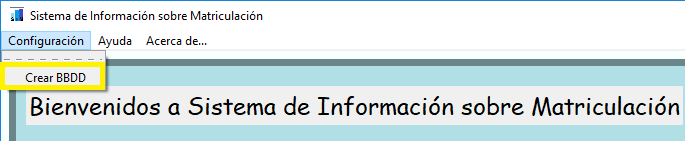
\includegraphics[width=0.9\textwidth]{crearBBDD}
		\caption{Botón de creación de la Base de Datos}\label{fig:crearBBDD}
	\end{figure}


Al pulsar sobre este botón se creará la Base de Datos y por consiguiente el fichero BBDD en la ruta donde estemos ejecutando la aplicación.
Si es la primera vez que pulsamos este botón, se creará con éxito; pero si ya existiera la BBDD, la aplicación nos mostraría un mensaje de \emph{Warning} como el de la figura \ref{fig:warningBBDD}. De esta forma, no se volverá a crear la Base de Datos y mantendremos nuestra BBDD anterior.

\begin{figure}%[!h]
		\centering
		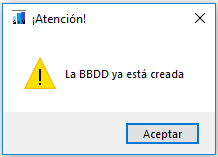
\includegraphics[width=0.5\textwidth]{warningBBDD}
		\caption{Mensaje de \emph{Warning} de BBDD ya creada}\label{fig:warningBBDD}
	\end{figure}



\subsection{Preprocesado de los ficheros Excel (.xls) descargados de \emph{Sigma}}

Una vez creada la BBDD, necesitamos introducir o meter los datos. Para esta labor, se utilizan ficheros de datos de matriculación de alumnos descargados de \emph{Sigma}.

Ya se han explicado los problemas que existen con estos tipos de ficheros, por esta razón, se deben parsear y preprocesar antes de añadir a la BBDD. Para esta tarea, contamos con el botón de \emph{Preprocesado}. Este botón se ubica en la pantalla principal de la aplicación, ya que es un botón que se utilizará con cierta normalidad y periodicidad. 

\begin{figure}%[!h]
		\centering
		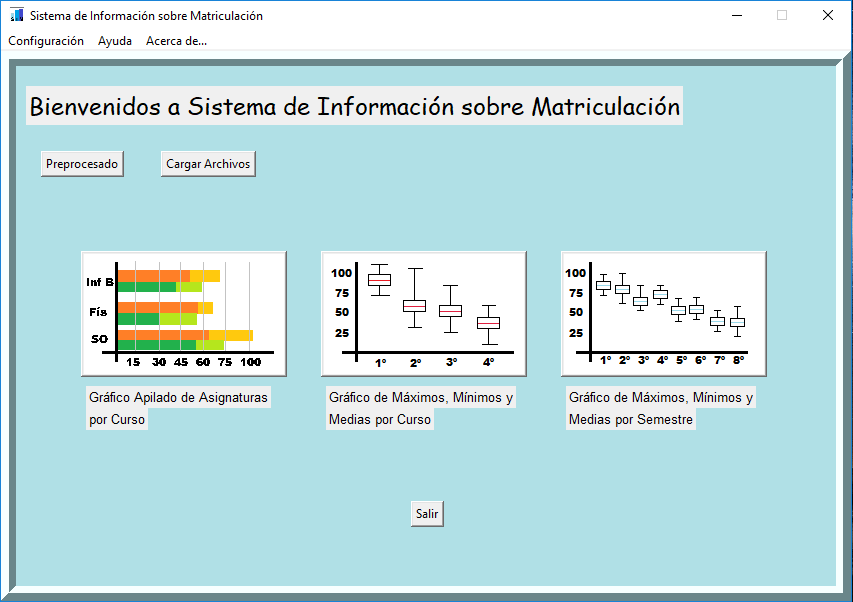
\includegraphics[width=\textwidth]{pantallaPrincipal}
		\caption{Pantalla principal de la aplicación}\label{fig:pantallaPrincipal}
	\end{figure}


Cuando pulsemos el botón de \emph{Preprocesado} (\ref{fig:pantallaPrincipal}), se mostrará una ventana del Sistema Operativo, donde se nos permitirá seleccionar archivos (.xls) únicamente (\ref{fig:ventanaSOxls}).


\begin{figure}%[!h]
		\centering
		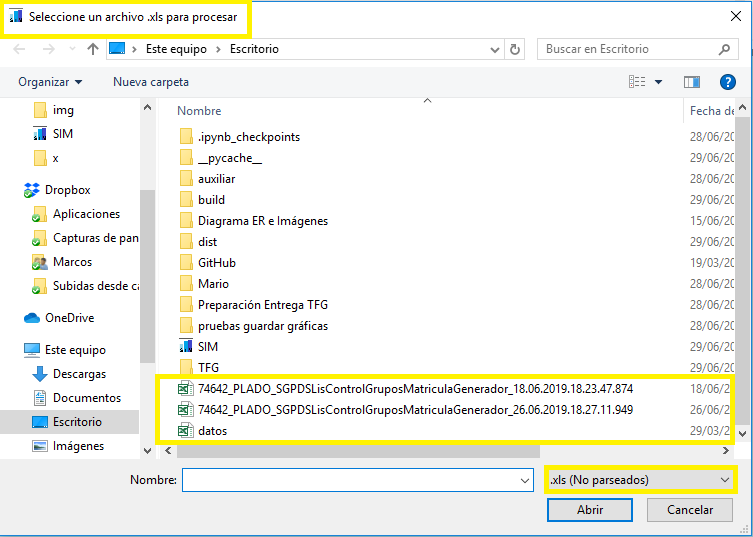
\includegraphics[width=\textwidth]{ventanaSOxls}
		\caption{Ventana del Sistema Operativo (seleccionar .xls)}\label{fig:ventanaSOxls}
	\end{figure}


Seleccionamos el archivo que deseemos (deben ser archivos descargados de \emph{Sigma}) y pulsamos abrir.
Una vez realizado esto, se generará en la misma ruta un fichero con extensión (.csv) corregido, modificado y preparado para la carga de datos en la BBDD. El resumen del proceso de preprocesado de ficheros sigma se puede apreciar en la figura  \ref{fig:sigmaAprocesado}.

\begin{figure}%[!h]
		\centering
		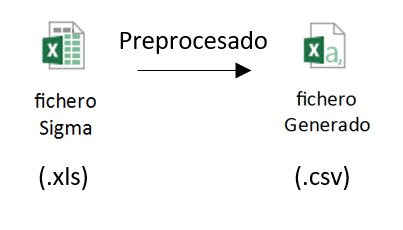
\includegraphics[width=0.5\textwidth]{sigmaAprocesado}
		\caption{Resumen de botón \emph{Preprocesado}}\label{fig:sigmaAprocesado}
	\end{figure}


\subsection{Carga de datos en la Base da Datos (BBDD)}

En este punto, ya podemos realizar la carga de datos. Para eso contamos con un botón de \emph{Cargar Archivos} situado también en la pantalla principal de la aplicación (\ref{fig:pantallaPrincipal}).

De la misma forma que el anterior paso, cuando pulsamos este botón, se mostrará una ventana del Sistema Operativo, donde se nos permitirá seleccionar archivos (.csv) únicamente (\ref{fig:ventanaSOcsv}).

\begin{figure}%[!h]
		\centering
		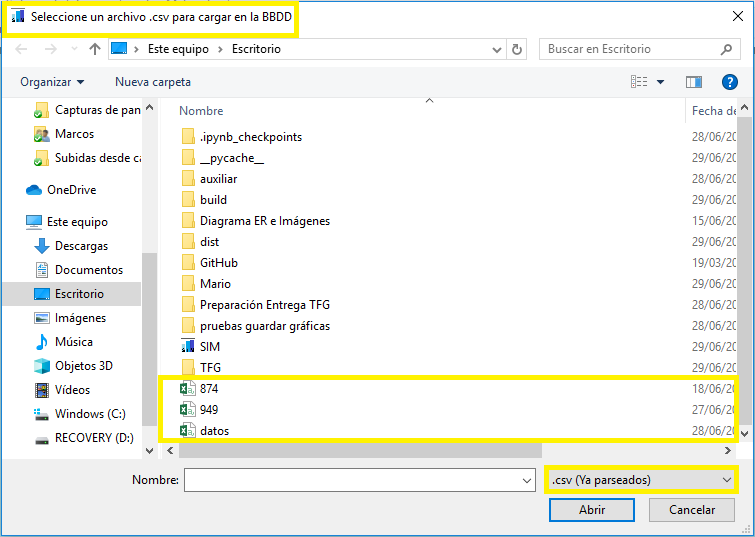
\includegraphics[width=\textwidth]{ventanaSOcsv}
		\caption{Ventana del Sistema Operativo (seleccionar .csv)}\label{fig:ventanaSOcsv}
	\end{figure}


Seleccionamos el archivo que se ha generado en el paso anterior y pulsamos abrir. Una vez realizado esto, se procederá a realizar la carga de todos los datos del fichero a la BBDD siguiendo las normas de claves primarias definidas en el modelo ER de la aplicación. El resumen del proceso de carga de datos se puede apreciar en la figura \ref{fig:procesadoABBDD}. 

\begin{figure}%[!h]
		\centering
		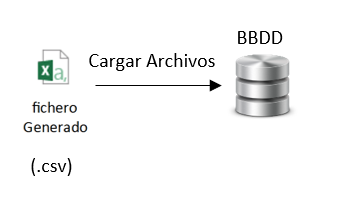
\includegraphics[width=0.5\textwidth]{procesadoABBDD}
		\caption{Resumen de botón \emph{Cargar Archivos}}\label{fig:procesadoABBDD}
	\end{figure}



\subsection{Selección y personalización de los gráficos}

En este punto, ya contamos con información o datos suficientes para realizar los diferentes tipos de gráficos.
Por lo tanto pulsamos en una de las imágenes (botones) de la pantalla principal (\ref{fig:pantallaPrincipal}) de los 3 tipos de gráficos (el primero por ejemplo) y se nos abrirá una nueva ventana (\ref{fig:ventana1}).

\begin{figure}%[!h]
		\centering
		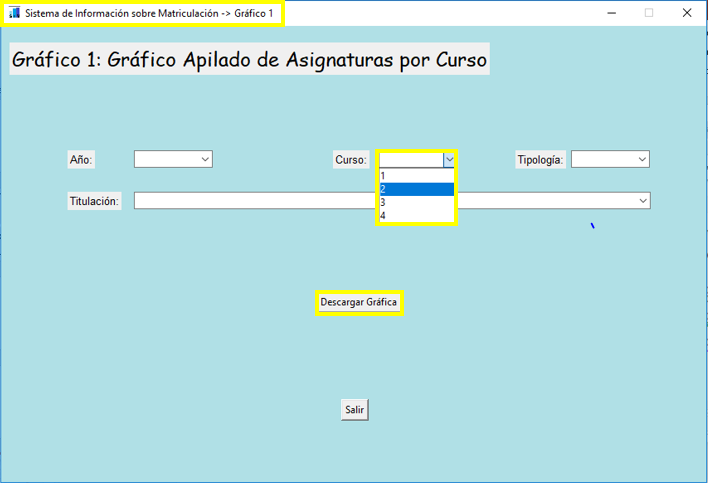
\includegraphics[width=\textwidth]{ventana1}
		\caption{Ventana secundaria para configurar el gráfico 1}\label{fig:ventana1}
	\end{figure}

En esta ventana, se muestran una serie de desplegables con la información necesaria para que el usuario seleccione y escoja los parámetros para generar el tipo de gráfico específico que desee. Hay que destacar que en cada desplegable se muestra toda la información diferente que se encuentre en la BBDD.

	
Para obtener correctamente el gráfico, es necesario seleccionar una opción de cada desplegable. En este ejemplo, es decir, en el tipo de gráfico 1, es necesario seleccionar cuatro parámetros, que son los siguientes (\ref{fig:ventana1}):


\begin{itemize}
\item \textbf{Año.} Año académico que se desea visualizar en la gráfica.
\item \textbf{Curso.} Curso que se desea visualizar. Los posibles valores son cuatro cursos (1º, 2º, 3º y 4º).
\item \textbf{Tipología.} Tipología académica que se quiere visualizar. Los posibles valores son dos tipologías (Teoría y Prácticas).
\item \textbf{Titulación.} Nombre de la titulación o plan que se desea obtener el gráfico.
\end{itemize}
   
Una vez hayamos escogido estos cuatro parámetros, podemos proceder a la descarga del gráfico.


Como se aprecia en la figura \ref{fig:ventana2}, para los tipos de gráfico 2 y 3, es necesario seleccionar únicamente dos parámetros, explicados anteriormente, que son los siguientes:

\begin{itemize}
\item \textbf{Año.}
\item \textbf{Titulación.}
\end{itemize}
  
\begin{figure}%[!h]
		\centering
		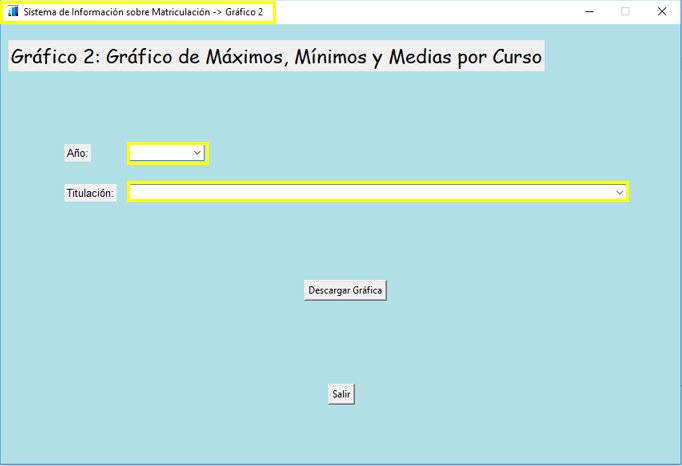
\includegraphics[width=\textwidth]{ventana2}
		\caption{Ventana secundaria para configurar el gráfico 2}\label{fig:ventana2}
	\end{figure}
	
	
\subsection{Descarga de los gráficos}

Para descargar el gráfico, únicamente debemos pulsar el botón de \emph{Descargar Gráfica} situado en las ventanas secundarias de configuración de los diferentes tipos de gráficos. Este botón se puede apreciar en las figuras \ref{fig:ventana1} y \ref{fig:ventana2}.

Una vez pulsado dicho botón se descargará la gráfica con extensión (.png) en la ruta donde estemos ejecutando la aplicación.
La nomenclatura de estos archivos es la siguiente:
 
\begin{itemize}
\item \textbf{Gráfico 1.} \emph{Grafica1} seguido de una \emph{T} (tipología teoría) o una \emph{P} (tipología prácticas), seguido de \emph{\_curso\_x} (siendo \emph{x} el tipo de curso seleccionado y por último el plan o titulación.
\item \textbf{Gráfico 2.} \emph{Grafica2\_cursos\_} seguido del plan o titulación seleccionado.
\item \textbf{Gráfico 3.} \emph{Grafica3\_semestres\_} seguido del plan o titulación seleccionado.
\end{itemize}



\subsection{Gráficos obtenidos}

Los diferentes gráficos principales que se pueden obtener gracias a la aplicación son los siguientes: \ref{fig:grafico1T}, \ref{fig:grafico1P}, \ref{fig:grafico2} y \ref{fig:grafico3}.


\begin{figure}%[!h]
		\centering
		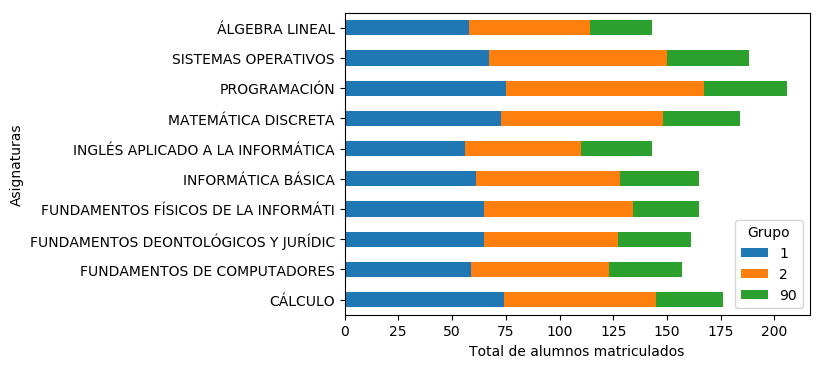
\includegraphics[width=\textwidth]{grafico1T}
		\caption{Gráfico 1: Gráfico Apilado de Asignaturas de año 2018-2019 de 1º de Grado en Ingeniería Informática de Tipología Teoría}\label{fig:grafico1T}
	\end{figure}


\begin{figure}%[!h]
		\centering
		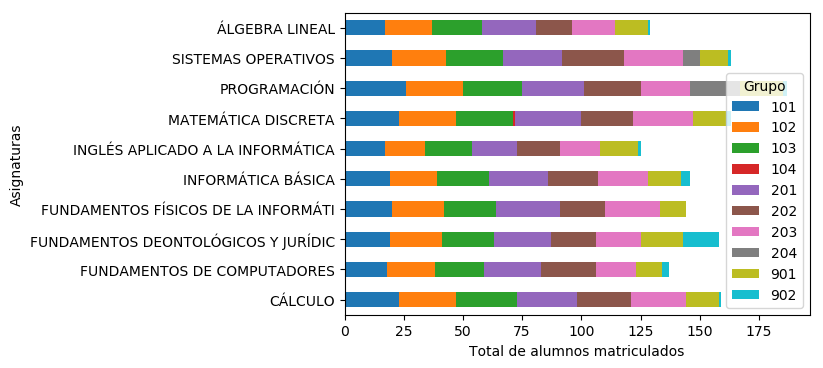
\includegraphics[width=\textwidth]{grafico1P}
		\caption{Gráfico 1: Gráfico Apilado de Asignaturas del año 2018-2019 de 1º del Grado en Ingeniería Informática de Tipología Prácticas}\label{fig:grafico1P}
	\end{figure}

\begin{figure}%[!h]
		\centering
		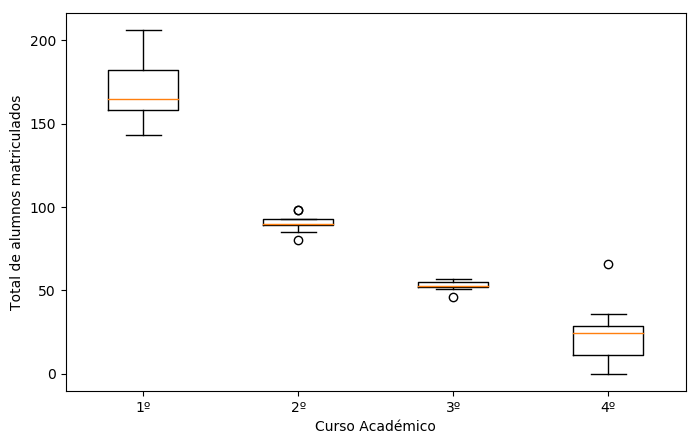
\includegraphics[width=0.8\textwidth]{grafico2}
		\caption{Gráfico 2: Gráfico Apilado de Máximos, Mínimos y Medias por Curso del año 2018-2019 del Grado en Ingeniería Informática}\label{fig:grafico2}
	\end{figure}

\begin{figure}%[!h]
		\centering
		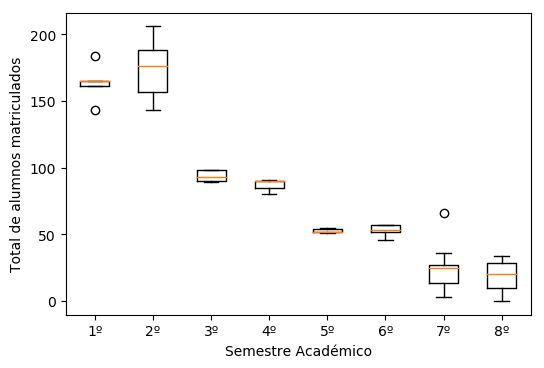
\includegraphics[width=0.8\textwidth]{grafico3}
		\caption{Gráfico 3: Gráfico Apilado de Máximos, Mínimos y Medias por Semestre del año 2018-2019 del Grado en Ingeniería Informática}\label{fig:grafico3}
	\end{figure}


\subsection{Otras funcionalidades}

Hay que señalar que la aplicación cuenta con una opción de \emph{Ayuda} en el menú superior. Al pulsar este botón se desplegarán dos opciones (\emph{Ayuda Local} y \emph{Ayuda Web}) como se aprecia en la figura \ref{fig:ayuda}. Si pulsamos la primera opción, nos abrirá el (.pdf) de ayuda que se incorpora en la aplicación; y si pulsamos la segunda opción nos abrirá el mismo (.pdf) de ayuda pero dicho archivo se encuentra subido en el repositorio de GitHub. De esta manera, mediante esta segunda opción, se podría actualizar la información relevante a la \emph{Ayuda} de manera inmediata para el usuario.

\begin{figure}%[!h]
		\centering
		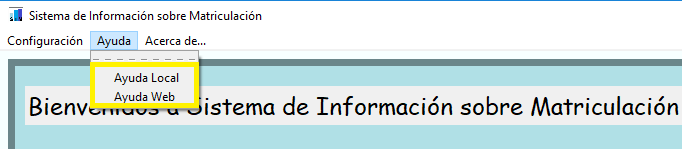
\includegraphics[width=0.8\textwidth]{ayuda}
		\caption{Opción de \emph{Ayuda}}\label{fig:ayuda}
	\end{figure}

Para finalizar, hay que comentar que la aplicación cuenta con un botón de \emph{Acerca de...}, situado a la derecha del botón de ayuda, como se aprecia en la figura \ref{fig:ayuda}.

Si pulsamos sobre este botón nos mostrará información relevante del proyecto (nombre, logotipo, autor, tutor, versión, licencia...etc) como se aprecia en la figura \ref{fig:acercaDe}.

\begin{figure}%[!h]
		\centering
		
\includegraphics[width=0.8\textwidth]{acercaDe}
		\caption{Contenido de \emph{Acerca de...}}\label{fig:acercaDe}
	\end{figure}


\bibliographystyle{plain}
\bibliography{bibliografiaAnexos}

\end{document}
